\documentclass[11pt]{article}
\usepackage[margin = 2cm]{geometry}

\usepackage{amsmath}
\usepackage{amsthm}
\usepackage{amssymb}
\usepackage{graphicx}
\usepackage{physics}

\usepackage{xcolor}
\definecolor{mycolor}{rgb}{.1, .30, .9}
\usepackage[colorlinks = true,
linkcolor = mycolor,
citecolor = mycolor,
urlcolor = mycolor]{hyperref}

\newtheorem{defn}{Def}
\newtheorem{prop}{Prop}
\newtheorem{thm}{Thm}
\newtheorem{rmk}{Remark}

\newcommand{\e}{\mathrm{e}}
\newcommand{\ii}{\mathrm{i}}
\renewcommand{\epsilon}{\varepsilon}
\newcommand{\Int}{\mathrm{Int}}

\begin{document}
\noindent\Large{Higher-form symmetries in the language of differential geometry} \\
\normalsize{\textbf{Ben McDonough}}\\\
\normalsize{\today}

\tableofcontents

\section{Introduction}
In recent years, the concept of symmetry in quantum field theory has been significantly generalized. Ordinary (0-form) symmetries act on pointlike operators and are associated with codimension-1 topological operators. Higher-form symmetries extend this paradigm by acting on extended objects, such as line or surface defects, and are characterized by higher-codimension topological operators. In these notes, we will explain the basics of higher-form symmetries and the differential geometry concepts needed to pursue further reading. The main sources for these notes are \cite{luo2024lecture, brennan2023introductiongeneralizedglobalsymmetries}. The paper that introduced and consolidated many of these ideas is \cite{Gaiotto_2015}, and it is also quite readable.
Lastly, we will explore the application of generalized symmetries to E\&M.

\section{Noether's theorem}
Consider a QFT with action $S$. An ordinary (0-form) symmetry of this QFT is a
transformation
\begin{align}
y^\mu &= x^{\mu} + \epsilon^\alpha \frac{\partial x^\mu}{\partial \epsilon^\alpha} &  \phi'  = \mathcal F(\phi) &\approx \phi + \epsilon^\alpha\frac{\partial \mathcal F}{\partial \epsilon^\alpha}
\end{align}
under which the action is invariant. To compute the variation of the action
explicitly, we first find the Jacobian of the transformation in the limit of
small $\epsilon$:
\begin{align}
\det\left(\left[\frac{\partial y^\nu}{\partial x^\mu}\right]_{\mu \nu}\right) \approx \det\left(\e^{\left[\frac{\partial}{\partial x^\nu}\left(\epsilon^\alpha\frac{\partial x^\mu}{\partial \epsilon^\alpha}\right)\right]_{\mu \nu}}\right) = \e^{\Tr\left[\frac{\partial}{\partial x^\nu}\left(\epsilon^\alpha\frac{\partial x^\mu}{\partial \epsilon^\alpha}\right)\right]_{\mu \nu}} \approx 1+\frac{\partial}{\partial x^\mu}\left[\epsilon^\alpha\frac{\partial x^\mu}{\partial \epsilon^\alpha}\right] .
\end{align}
This gives the determinant to $\mathrm O(\epsilon)$. Next, the partial
derivatives transform as
\begin{align}
  \frac{\partial y^\nu}{\partial x^\mu} = \delta_{\mu\nu} + \frac{\partial}{\partial x^\mu}\left[\epsilon^\alpha \frac{\partial x^\nu}{\partial \epsilon^\alpha}\right] ,
\end{align}
so to first order in $\epsilon$,
\begin{align}
  \frac{\partial}{\partial y^\nu} = \frac{\partial x^\mu}{\partial y^\nu}\frac{\partial}{\partial x^\mu} =  \frac{\partial}{\partial x^\nu} - \frac{\partial}{\partial x^\nu}\left[\epsilon^\alpha \frac{\partial x^\mu}{\partial \epsilon^\alpha}\right]\frac{\partial}{\partial x^\mu} .
\end{align}
Plugging these into the action, we find
\begin{align}
  \delta S & = \int \dd^{d+1} y \mathcal L\left(\phi', \frac{\partial \phi'}{\partial y^\mu}\right) - \int \dd^{d+1} x \mathcal L\left(\phi, \frac{\partial \phi}{\partial x^\mu}\right) \notag\\
  &= \int \dd^{d+1}x \left(1 + \partial_\mu \epsilon^\alpha \frac{\partial x^\mu}{\partial \epsilon^\alpha}\right)\mathcal L\left(\phi + \epsilon^\alpha\frac{\partial \mathcal F}{\partial \epsilon^\alpha}, (\delta_{\mu \nu} - \partial_\mu \epsilon^\alpha\frac{\partial x^\nu}{\partial \epsilon^\alpha})\partial_\mu \left[\phi + \epsilon^\alpha\frac{\partial \mathcal F}{\partial \epsilon^\alpha}\right]\right) - \mathcal L(\phi,\partial_\mu \phi) .
\end{align}
Since we can take $\partial_\mu \epsilon^\alpha = 0$ and then bring
$\epsilon^\alpha$  outside of the integral, this means that the terms not
containing derivatives of $\epsilon^\alpha$ must cancel. We can just keep the
terms with $\partial_\mu \epsilon^\alpha$ in the expansion, and we find
\begin{align}
  \delta S &= \int \dd^{d+1} x \left[ \frac{\partial \mathcal L}{\partial (\partial_\nu\phi)}\frac{\partial \mathcal F}{\partial \epsilon^\alpha}\partial_\nu\epsilon^\alpha - \frac{\partial \mathcal L}{\partial (\partial_\nu\phi)}\partial_\mu \epsilon^\alpha \frac{\partial x^\nu}{\partial \epsilon^\alpha}\partial_\mu \phi + \partial_\mu \epsilon^\alpha\frac{\partial x^\mu}{\partial \epsilon^\alpha} \mathcal L \right] \\
  &= \int \dd^{d+1} x j_\alpha^\nu \partial_\nu \epsilon^\alpha = 0,
\end{align}
where we introduced the current
\begin{align}
  j_\alpha^\nu &= \frac{\partial \mathcal L}{\partial (\partial_\nu \phi)}\frac{\partial \mathcal F}{\partial \epsilon^\alpha} + \frac{\partial x^\mu}{\partial \epsilon^\alpha}\underbrace{\left[\mathcal L\delta_{\mu \nu} - \frac{\partial \mathcal L}{\partial (\partial_\nu \phi)}\partial_\mu \phi\right]}_{T_{\mu \nu}}
\end{align}
and also identified the stress tensor $T_{\mu \nu}$.
Using integration by parts, we find
\begin{align}
\int j_\alpha^\nu \partial_\nu \epsilon^\alpha &= - \int \partial_\nu j_\alpha^\nu \epsilon^\alpha = 0.
\end{align}
Then since $\epsilon^\alpha$ is arbitrary, we must have the continuity equation
\begin{align}
\partial_\mu j_\alpha^\nu &= 0.
\end{align}
This conserved current
leads to a conserved charge
\begin{align}
Q(t) = \int_M \dd^dx j_\alpha^0,
\end{align}
where $M$ is a spatial slice of spacetime at time $t$.
This charge is conserved because
\begin{align}
  \dot Q = \int_{M} \dd^d x \partial_0j_\alpha^0 &= -\int_M \dd^d x \partial_i j_\alpha^i = \int_{\partial M} \dd^{d-1}x j_\alpha^i \cdot \hat n = 0,
\end{align}
where $i$ refers to Euclidean indices and we assume that $j_\alpha = 0$ on
$\partial M$.

\section{Higher-form symmetry}
First, we notice that a fixed time $t$ is the same as a 3D slice of 4D
spacetime, which we call $\Sigma_3$. In this language the conserved charge is
defined by
\begin{align}\label{eq:ordinary_charge}
  Q_\alpha(\Sigma_3) = \int_{\Sigma_3} j_\alpha^\mu \hat n^\mu 
\end{align}
where $\hat n$ is the normal vector to $\Sigma_3$. If $\Sigma_3$ is a slice of
spacetime at a fixed time, then $\hat n = (1,0,0,0)$ and this reduces to the
ordinary definition of $Q(t)$. However, we notice that $\Sigma_3$ can just as
well be an arbitrary 3-submanifold of spacetime. What is the
analogous conservation law? Suppose that $M$ is a 4-submanifold with boundary, and $\partial M = \Sigma_3 \sqcup \Sigma_3'$ with
opposite orientations. Then
\begin{align}
Q_\alpha(\Sigma_3) - Q_\alpha(\Sigma_3') = \int_{\Sigma_3}j_\alpha^\mu n^\mu - \int_{\Sigma_3'}j_\alpha^\mu n^\mu = \int_{\partial M}j_\alpha^\mu n^\mu = \int_{M}\partial_\mu j_\alpha^\mu = 0
\end{align}
This implies that $Q_{\alpha}$ is a \emph{topological invariant} in that it only
depends on the homology class of $\Sigma_3$.

In this language, we would call the global symmetry an \emph{ordinary} or
\emph{0-form} symmetry, and say that it acts on a \emph{codimension-1}
submanifold (in spacetime). Viewing charges as topological
invariants rather than conserved quantities will allow us to generalize to $p >
0$. 

\subsection{Riemannian geometry and the Hodge star}
To generalize this idea, we introduce the Hodge star. First we need to talk
about Riemannian structures. In the following, let $M$ denote spacetime.
A Riemannian structure is a 2-covector field $g \in \Omega^2(M)$ which restricts
on each tangent space $T_pM$ to an inner product.
A Riemannian structure allows us to canonically relate vector fields and
covector fields:
\begin{defn}[Musical isomorphisms]
  Let $\{E_i\}$ be an orthonormal frame for $T_pM$ for $p \in U$.
  Then if $j = j^i E_i$ is a vector field, we define the dual covector
  field to be
  \begin{align}
    j &= j^i E_i \Rightarrow j^\flat = j_i \epsilon^i \\
    J &= J_i \epsilon^i \Rightarrow J^\sharp = J^iE_i
  \end{align}
  where $\epsilon^i = \langle E_i, \cdot \rangle_g$ is a covector.
  The raised/lowered index on $j$ is irrelevant because we are working in a
  basis where $g$ is diagonal. The musical isomorphisms correspond to raising
  and lowering the indices, hence the sharp and flat. It is clear that this
  definition is invariant under isometry, corresponding to a different choice of
  orthonormal frame.
\end{defn}


\begin{defn}
  Given $ \omega \in \Omega^k(M)$, the Hodge star is a map $*:\Omega^k(M) \to
  \Omega^{d+1-k}(M)$, where $*\omega$ is the unique form such that
  \begin{align}
    \omega \wedge *\eta \equiv \langle \omega, \eta \rangle_g \dd V_g
  \end{align}
 where 
  $\dd V_g$ is the Riemannian volume form.
\end{defn}
The Hodge star generalizes divergence in the following way:
\begin{prop}
  Given a vector field $j$, the divergence at $p$ is $(\div j)_p =
  \partial_ij^i$ where $\{x^i_p\}$ are a set of orthonormal coordinates at $p$.
  By orthonormal coordinates, we mean that $\left\{\frac{\partial}{\partial x^i_p}\right\}_i$ form an
  orthonormal basis for $T_pM$. In terms of the Hodge star, we have
  \begin{align}
\div j = *\dd*j^\flat .
\end{align}
This can be used to define the analogous divergence of a $p$-form.
\end{prop}

\begin{proof}
We have
\begin{align}
* j^\flat = j^i\epsilon_{i, i_1, \ldots, i_{d+1}} \dd x^{i_1} \wedge \ldots \wedge \dd x^{i_{d+1}}
\end{align}
Taking the exterior derivative,
\begin{align}
  \dd * j^\flat &= \frac{\partial j^i}{\partial x^j} \epsilon_{i, i_1, \ldots, i_{d+1}} \dd x^j \wedge \dd x^{i_1} \wedge \ldots \wedge \dd x^{i_{d+1}}
  = \frac{\partial j^i}{\partial x^i}\dd V_g
\end{align}
Then the result follows from $* \dd V_g = 1$.
\end{proof}

\begin{prop}[Stokes' theorem for divergence]
\begin{align}
  \int_M (\div X)\dd V_g = \int_{\partial M}\langle  N, X \rangle_g
\end{align}
where $N$ is the unit normal vector field to $\partial M$.
\end{prop}

The notion of a unit normal vector field just generalizes the normal vector
$\hat n$. The
Riemannian structure affords a decomposition of each tangent space of $M$ for $p
\in \partial M$ as
\begin{align}
  T_p M = T_p \partial M \oplus (T_p \partial M)^\perp
\end{align}
and then we can choose a unique normalized vector in $(T_p M)^\perp$ to call
$N_p$. Since $g$ is smooth and $\partial M$ is a smooth submanifold, the
resulting vector field $N$ is smooth.

\begin{prop}\label{prop:outflow}
  Let $\Sigma$ be a codimension-1 submanifold with a unit normal vector field
  $N$. Then
  \begin{align}
    * X^\flat = \langle N, X \rangle \dd V_{\tilde g}
  \end{align}
  where $\dd V_{\tilde g} = i_N \dd V_{g}$ is the volume form induced on $\Sigma$.
\end{prop}
\begin{proof}
  We choose the oriented orthonormal basis $\epsilon^0 = N^\flat, \epsilon^1, \ldots, \epsilon^{d-1}$. Then
\begin{align}
*X^\flat|_{\Sigma} = X^i \epsilon_{i, i_1, \ldots, i_{d-1}}\epsilon^{i_1} \wedge \ldots \wedge \epsilon^{i_{d-1}}|_{\Sigma} = X^0 \epsilon^{1} \wedge \ldots \wedge \epsilon^{d-1}
\end{align}
where the volume form induced on $\Sigma$ is exactly $\epsilon^1 \wedge \ldots
\wedge \epsilon^{d-1} = i_N(\dd V_g)$ and $X^i = \epsilon^i(X) = \langle
(\epsilon^i)^\sharp, X\rangle$.
\end{proof}
From this, the divergence theorem follows as a consequence of Stokes' theorem
\begin{align}
\int_M \div X \dd V_g = \int_M \dd * X^\flat = \int_{\partial M} * X^\flat = \int_{\partial M}\langle  X, N \rangle_g \dd V_{\tilde g}
\end{align}

\subsection{$p$-form currents}

\begin{defn}
We will define the generalized continuity equation for a $p+1$-form current $j$:
\begin{align}
\dd * j = 0
\end{align}
and we will call such a current co-closed.
\end{defn}
\begin{rmk}
  The reason for calling this condition co-closure is that $*\dd* = \pm \dd^\dagger$
  with respect to the $L^2$ inner product on forms (for a closed, compact
  manifold $M$):
  \begin{align}
    \langle \omega, \dd\eta  \rangle &= \int_M \langle \omega, \dd \eta\rangle_g   \dd V_g
                                     = \pm \int_M \dd \eta \wedge * \omega 
                                       = \pm\int_M\eta \wedge \dd * \omega\notag\\
                                       &
                                     = \pm \int_M \eta \wedge ** \dd * \omega
                                     = \pm \int_M \langle  \eta, * \dd * \omega \rangle_g \dd V_g
    = \pm \langle  * \dd * \omega, \eta \rangle
  \end{align}
  where we used $** = \pm 1$ depending on the degree of the forms.
\end{rmk}

Then we can define the generalized conserved charge
\begin{defn}
  Given a codimension-$p+1$ manifold $\Sigma$ and a $p+1$-form current $j$, define
  \begin{align}
    Q(\Sigma) &= \int_{\Sigma} *j
  \end{align}
\end{defn}
To see how this definition reduces to the previous one when $j$ is a vector
field (i.e. $p = 0$), we apply
Prop.~\ref{prop:outflow} to find
\begin{align}
Q(\Sigma_3) = \int_{\Sigma_3}*j^\flat = \int_{\Sigma_3}\langle N, j\rangle_{g}\dd V_{\tilde g},
\end{align}
which is identical to Eq.~\eqref{eq:ordinary_charge}. We can see that this
generalizes to $p$-forms by computing the magnitude of the projection of
$j^\sharp$ onto directions orthogonal to the immersed submanifold $\Sigma$,
just like the notion of flux through a surface.

Importantly, generalized symmetries give rise to topological invariants. Suppose
that $\Sigma, \Sigma'$ bound a codimension-$p$ manifold $M$, i.e. $\partial M = \Sigma \sqcup \Sigma'$. Then
\begin{align}
  Q(\Sigma) - Q(\Sigma') = \int_{\partial M}* j = \int_{M}\dd * j = 0 \ .
\end{align}
Therefore $Q(\Sigma) = Q([\Sigma])$, where $[\Sigma]$ is the homotopy class of
$\Sigma$. Furthermore, if $\beta$ is a codimension-$p+2$ form and $*j' = *j + \dd \beta$, then
\begin{align}
Q'(\Sigma) - Q(\Sigma) = \int_{\Sigma}\dd \beta = \int_{\partial \Sigma}\beta = 0
\end{align}
since we assumed that $\Sigma$ was a manifold without boundary. Thus, the
generalized charge is actually just the duality pairing between homology
and cohomology, i.e. $Q(\Sigma) \equiv [*j]([\Sigma])$, where $[*j]$ is the
cohomology class of $*j$.

\section{Observables in QFT}
The discussion so far has been purely classical, and when translating from
currents to charged observables and unitary operators, the reframing of
symmetries as topological invariants becomes very helpful.

First, a brief reminder about observables in QFT. Given a Hamiltonian $H$, the
path integral is derived through Trotterization:
\begin{align}
  \bra{\phi_i}\e^{\ii H(t+ \ii \epsilon)}\ket{\phi_f} &= \int_{\phi_i(0)}^{\phi_f(t)}\mathcal D[\phi]\e^{\ii S_\epsilon}
\end{align}
where $S_\epsilon$ is the appropriately regularized action. Using this prescription, we can compute a time-ordered
correlation function:
\begin{align}
  &\bra{0}\hat\phi_1(x_1, t_1) \ldots \hat \phi_n(x_n, t_n) \ket{0} \notag \\
  &= \lim_{\epsilon \to 0}\lim_{\substack{T_i \to -\infty\\ T_f \to \infty}}\frac{\bra{\phi_i}\e^{\ii H (T_i - t_1)(1- \ii \epsilon)}\hat \phi(x_1) \e^{\ii H(t_1 - t_2)(1 - \ii \epsilon)} \hat \phi(x_2) \ldots \hat \phi(x_n) \e^{-\ii HT_f(1+\ii \epsilon)}\ket{\phi_f}}{\bra{\phi_i}\e^{\ii H(T_i - T_f)(1+ \ii \epsilon)}\ket{\phi_f}} \\
  &= \lim_{\epsilon \to 0}\frac{\int_{\phi_i}^{\phi_f}\mathcal D[\phi]\phi(t_1, x_1)\phi(t_2, x_2)\ldots \phi(t_n, x_n)\mathcal D[\phi]\e^{\ii S_\epsilon}}{\int_{\phi_i}^{\phi_f}\mathcal D[\phi]\e^{\ii S_\epsilon}},
\end{align}
for \emph{any} $\phi_i, \phi_f$, so we usually integrate them out.
We also assumed the system is gapped, so
\begin{align}
  \lim_{t \to \infty}\e^{-\ii H (t-\ii \epsilon)}\ket{\phi} &= \lim_{t \to \infty}\sum_{n} \ket{n} \e^{-\ii E_n (t - \ii \epsilon)}\braket{n}{\phi} \notag\\
  &= \braket{0}{\phi}
\end{align}
We see that the path integral naturally forces time-ordering under the
expectation value. 

\subsection{Symmetry defects}
We will call a family $\{O_i\}_i$ of observables charged under a symmetry group
$G$, acting by a representation $U_g$, if
\begin{align}
  U_g^\dagger O_i U_{g} = R_{i}^j(g)O_j \label{eq:charged}
\end{align}
for some representation $R$ of $G$. From above, since $U_g$ commutes with $H$,
we have
\begin{align}
  \langle  U_g^\dagger(t_1)O_i(t)U_g(t_2) \rangle = 
  \langle  U_g^\dagger(t_1')O_i(t)U_g(t_2') \rangle
\end{align}
for any $t_1 < t < t_2$ and $t'_1 < t < t_2'$. However, by \eqref{eq:charged},
this is not true for $t_1 < t$ and $t'_1 > t$. If we imagine each time $t$ as
specifying a 3d slice $\Sigma_3$ of spacetime, then this means we can
topologically deform $\Sigma_3$, but $O_i$ acts like a puncture in spacetime,
through which $\Sigma_3$ cannot be smoothly deformed. Taking advantage of the
ability to deform $\Sigma_3$ in the time direction as well, we can deform
$\Sigma_3$ and $\Sigma_3'$ (corresponding to $t_2$) until $\Sigma_3 \cup
\Sigma_3'$ form the boundary of an arbitrarily small manifold $M$ containing the
point at which $O_i$ acts, as shown in Fig.~\ref{fig:deformation}.
\begin{figure}[hbt!]
  \centering
  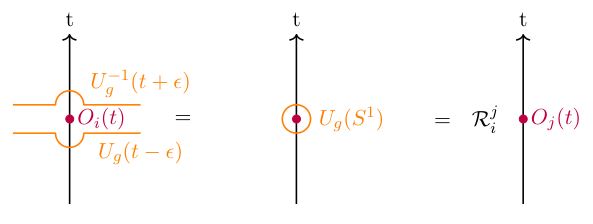
\includegraphics[width =.6\textwidth]{symmetry_homotopy.png}
  \caption{Figure showing how to interpret a zero-form
    symmetry as a homological pairing and a charged operator $O_i$ as a
    point-like singularity.}
  \label{fig:deformation}
\end{figure}

This is our first example of \emph{linking}:
\begin{prop}
Given a $p$-dimensional submanifold $M$ and a codimension $p+1$ submanifold $N$, we define a \emph{linking number} as follows: choose a submanifold $M'$ (resp. $N'$) such that $M = \partial M'$ (resp. $N = \partial N'$), and define
  \begin{align}
\langle  M, N \rangle \equiv \Int(M, N')  = \Int(M', N)
  \end{align}
  where $\Int$ counts the number of oriented intersections between the two
  submanifolds. It is a theorem that this number is a homotopy invariant of $M$
  and $N$.
\end{prop}

In the case of an ordinary symmetry, $p = 0$ and $O_i$ which is point-like links
with the codimension-1 manifold $\Sigma_3$ if $\Sigma_3$ bounds a manifold
containing the support of $O_i$.

To generalize this, given a $p+1$-form current $j$, a codimension-$p+1$
submanifold $\Sigma$, and a Lie algebra element $\mathfrak g$, we define the
symmetry defect operator to be
\begin{align}
  U_g(\Sigma) \equiv \e^{\mathfrak g Q(\Sigma)} = \e^{\mathfrak g \int_{\Sigma}*j}.
\end{align}
Then we will use the linking from before to define a general charged operator:
\begin{defn}
  Let $\Sigma$ be any codimension $p+1$ submanifold. We call $\{O_i(M)\}$
  charged if for $p$-submanifold $M$ which links once with $\Sigma$, we have
  \begin{align}
    \langle \mathcal T\{U_g(\Sigma)O_i(M)\}\rangle = R_i^j(g)\langle \mathcal T\{O_j(M)\}\rangle
  \end{align}
  where $O_i(M)$ is supported on $M$, and we used $\mathcal T$ to emphasize the
  time-ordering under the expectation value.
\end{defn}
Notice that the time-order captures the conjugation of $O_i$ by $U_g$ that we
saw in the zero-form case when $M$ is point-like and $\Sigma$ is a submanifold
containing $\Sigma$! This is also why we call the symmetry $p-$form; because the
operators which are charged under the symmetry are $p$-dimensional.

\section{Application: E\&M}
We will illustrate these concepts in matter-free electromagnetism. First, we
have seen how to write the Maxwell action as
\begin{align}
  S = -\frac{1}{4e^2}\int \dd^4 x F^{\mu\nu}F_{\mu \nu} = -\frac{1}{2e^2}\int \langle  F, F \rangle_{g} = -\frac{1}{2e^2}\int F \wedge *F .
\end{align}
We recognized the presence of the Riemannian inner product in the action $S$ and
re-wrote it in terms of the Hodge-star! The field strength tensor $F$ is defined
as $F_{\mu \nu} = \partial_\mu A_\nu - \partial_\nu A_\mu$, which can be written
as a 2-form in coordinate-free notation as
\begin{align}
F = \dd A
\end{align}
where $\dd$ is the exterior derivative. To find the classical equations of
motion, we vary the action with respect to $A$:
\begin{align}
  \delta S &= -\frac{1}{2e^2}\int \dd \delta A \wedge *F + F \wedge * \dd \delta A \notag\\
  &= -\frac{1}{e^2}\int \dd \delta A \wedge *F \notag\\
  &= -\frac{1}{e^2}\int \left[ \dd (\delta A \wedge *F) + \delta A \wedge \dd *F \right] \notag\\
  &= -\frac{1}{e^2} \int \delta A \wedge \dd *F
\end{align}
where we used integration by parts and the symmetry of the $ \cdot \wedge * \cdot= \langle
\cdot, \cdot  \rangle_g$ operator. This shows that
\begin{align}
\frac{\delta S}{\delta A} = -\frac{1}{e^2} \dd *F = 0
\end{align}
so $j = F$ is the co-closed 2-form current! What is the corresponding symmetry
operator? We have
\begin{align}
Q(\Sigma_2) = \int_{\Sigma_2} *F
\end{align}
The operator which is charged under this symmetry is the Wilson line operator.
Given a closed 1-submanfold (a line) $\gamma$, this is defined as
\begin{align}
  W_q(\gamma) = \exp\left(\ii  q\int_\gamma A\right)
\end{align}
We remember from undergrad E\&M that the term added to the action to couple to a
charge $q$ is simply
\begin{align}
- q\int \dd t A \cdot \dot x = -q\int_\gamma A
\end{align}
so the Wilson loop corresponds to inserting the worldline $\gamma$ of a charge
$q$. It turns out that $Q$ is just Gauss's law. To see how these operators link,
consider the action in the presence of charge:
\begin{align}
  S' = -\frac{1}{2e^2}\int F \wedge *F + 2e^2 q A \wedge \delta_\gamma
\end{align}
where $\delta_\gamma$ is a 3-form $\delta$-function on the loop $\gamma$.
Carrying out the variation again, we now find that
\begin{align}
  \delta S' = \int \delta A \wedge \left(-\frac{1}{e^2}\dd *F + q\delta_\gamma\right) = 0 \implies \dd * F = qe^2\delta_\gamma
\end{align}
Therefore the value of the charge is
\begin{align}
Q(\Sigma_2) = \int_{\Sigma_2} *F = \int_{\Sigma_3} \dd *F = qe^2\int_{\Sigma_3}\delta_\gamma = qe^2 \langle  \Sigma_2 , \gamma\rangle
\end{align}
where we chose $\partial \Sigma_3 = \Sigma_2$ and applied Stokes' theorem. We
can see that this is just the linking number, confirming that
$W_q(\gamma)$ is charged under the symmetry! Furthermore, since $Q(\Sigma_2)$
measures the amount of charge within $\Sigma_2$, we can identify this charge
with Gauss's law, and the corresponding symmetry as conservation of field lines.

Lastly, we remark on EM duality. Using $\dd^2 = 0$, we see that $\dd F = \dd^2A
= 0$, also known as the Bianchi identity. Since $** = \pm 1$, this gives another
conserved 2-form current $*F$ corresponding to conservation of magnetic field
lines. The corresponding dual symmetry operators are known as t'Hooft loops.

\section{Coupling to gauge fields}
The principal way to study an ordinary symmetry is to couple it to a 1-form
gauge field. Intuitively, domains in the gauge field become domains of the
symmetry. To generalize this, we can see that a $p+1$-form current naturally
couples to a $p+1$-form gauge field:
\begin{align}
  S_{\mathrm{int}} = \int A \wedge * j
\end{align}
What we need to verify is that the action is invariant under a gauge
transformation $A \mapsto A + \dd \lambda$, where $\lambda$ is a $p$-form. We
see that
\begin{align}
  \delta S_{\mathrm{int}} = \int \dd \lambda \wedge * j = (-1)^{p+1}\int \lambda \wedge \dd * j = 0,
\end{align}
so the invariance of this ``minimal coupling'' under gauge transformations is
implied by the co-closure condition.

\bibliographystyle{plain}
\bibliography{thebib}

\end{document}
